%%%%%%%%%%%%%%%%%%%%%%%%%%%%%%%%%%%%%%%%%%%%%%%%%%%%%%%%%%%%%%%%%%%%%%
% How to use writeLaTeX: 
%
% You edit the source code here on the left, and the preview on the
% right shows you the result within a few seconds.
%
% Bookmark this page and share the URL with your co-authors. They can
% edit at the same time!
%
% You can upload figures, bibliographies, custom classes and
% styles using the files menu.
%
%%%%%%%%%%%%%%%%%%%%%%%%%%%%%%%%%%%%%%%%%%%%%%%%%%%%%%%%%%%%%%%%%%%%%%

\documentclass[12pt]{article}

\usepackage{sbc-template}

\usepackage{graphicx,url}

%\usepackage[brazil]{babel}   
\usepackage[utf8]{inputenc}  
\usepackage{booktabs}
\usepackage{listings}
     
\sloppy

\title{Instructions for Authors of SBC Conferences\\ Papers and Abstracts}

\author{Matheus I. B. Santos\inst{1}, Andre L. L. Aquino\inst{2}, \\ Joubert de Castro Lima\inst{2}, Cristopher G. de S. Freitas\inst{2}}

\address{
Instituto de Computação -- Universidade Federal de Alagoas (UFAL)\\ Maceio, AL – Brazil
\nextinstitute
  Laboratório de Computação Científica e Análise Numérica (LaCCAN)\\
  Universidade Federal de Alagoas (UFAL) – Maceio, AL – Brasil
\nextinstitute
Federal University of Ouro Preto\\ R. Diogo de Vasconcelos, 122 – Ouro Preto, MG – Brasil
\email{\{matheus.inacio, alla, cristopher\}@laccan.ufal.br, joubertlima@gmail.com}
}

\begin{document} 

\maketitle

\begin{abstract}
  This meta-paper describes the style to be used in articles and short papers
  for SBC conferences. For papers in English, you should add just an abstract
  while for the papers in Portuguese, we also ask for an abstract in
  Portuguese (``resumo''). In both cases, abstracts should not have more than
  10 lines and must be in the first page of the paper.
\end{abstract}
     
\begin{resumo} 
  Este meta-artigo descreve o estilo a ser usado na confecção de artigos e
  resumos de artigos para publicação nos anais das conferências organizadas
  pela SBC. É solicitada a escrita de resumo e abstract apenas para os artigos
  escritos em português. Artigos em inglês deverão apresentar apenas abstract.
  Nos dois casos, o autor deve tomar cuidado para que o resumo (e o abstract)
  não ultrapassem 10 linhas cada, sendo que ambos devem estar na primeira
  página do artigo.
\end{resumo}


\section{Introdução}\label{intro}

Com crescimento de internet das coisa, áreas como sensoriamento têm crescido em conjunto, dado que aplicações desse tipo usam de dados coletados no ambiente. Por sua vez existe um problema comum quando falamos de integração em redes de sensores sem fio, que é focar no desenvolvimento da aplicação propriamente dita, já que nesses tipos de aplicações temos problema específicos da rede, problemas de infraestrutura, administração de uma rede heterogênea e até escalabilidade da rede~\cite{Heinzelman2004}.

Para abstração de operações de sistema, funcionalidades de baixo nível e dispor uma programação de alto nível, podemos usar um middleware. Geralmente, um middleware abstrai as complexidades do sistema ou hardware, permitindo que o desenvolvedor de aplicativos concentre todo o seu esforço na aplicação propriamente dita, sem a distração das preocupações ortogonais a nível do sistema operacional ou do hardware, assim como algumas peculiaridade que cada middleware pode trazer.

Nos últimos anos novos projetos vem trazendo novos middlewares para redes de sensores, dentre eles podemos citar ProActive~\cite{ProActive}, FamiWare~\cite{FamiWare}, C-MOSDEN~\cite{c-mosden}, SMEPP~\cite{SMEPP}, RAFDA~\cite{rafda}, PJ~\cite{PJ}, Jessica~\cite{jessica}, Open MPI~\cite{open-mpi}, P2P-MPI~\cite{p2p-mpi} e OpenIoT~\cite{openiot}. Dentre esses middleware, temos alguns grupos, que se distinguem em áreas de atuação, entre elas temos IoT, CoT e HPC, todo os middleware HPC possuem general-purpose computing, mas entre os demais grupo somente JCL possui essa funcionalidade, assim podemos dizer que ele pertence a uma intercção entre HPC e IoT.

Neste trabalho vamos abordar o uso do middleware JCL~\cite{Cimino2018}, para integração de redes de sensores, em paralelo fazer um comparativo com o uso do MQTT como Broker de integração. O middleware JCL é um projeto derivado do middleware HPC, assim herdando diversas funcionalidades de um middleware de sistema distribuído, assim como distributed storage, heterogeneity, simple deploy, general-purpose computing, low refactoring, task scheculer,  super-peer support, collaborative development e Performance and Scalability, com novo projeto propondo cobrir as necessidade  de aplicações IoT, novas funcionalidades foram adicionadas, podemos citar algumas, como service and privacy, context awareness e different programming models.

Dentre as funcionalidade que JCL herda do projeto HPC, temos algumas funcionalidades destaque, que não são encontradas em middlewares IoT ou CoT, como por exemplo, general-purpose computing (GPC), low refactoring (LR), task scheculer ou super-peer suport, GPC permite ao usuário executar tarefas de proposito geral derivadas de implementações java ou Android, e devido ao LR essas implementações não exigem grandes mudanças no código. Outra funcionalidade desejaval para um middleware é fault tolerance e sensing analytics, dentro os citados anteriormente temos o FamiWare com destaque para o quesito fault tolerance e o OpenIoT com um destaque para sensing analytics.

\section{Trabalhos Relacionados} \label{sec:firstpage}

\subsection{Middlewares}
\begin{table*}
  \caption{Comparison of middleware solutions}
  \label{tab:middlewares}
  \tiny
  \begin{tabular}{ccccccccccccccccl}
    \toprule
   Middleware & Type & SaP & CA & DPM & DS & H & SA & SD & FT & GPC & LR & TS & SP & CD & PaS\\
    \midrule
    FamiWare & IoT & * & * & - & - & * & - & - & ** & - & - & - & - & - & -\\
    C-MOSDEN & IoT & - & *** & - & - & * & - & ** & - & - & - & - & - & - & -\\ 
    SMEPP & IoT & *** & * & - & - & * & - & - & - & - & - & - & - & - & -\\ 
    JCL & IoT-HPC & ** & ** & *** & *** & * & - & ** & - & *** & *** & *** & *** & *** & ***\\
    ProActive & HPC & * & - & - & - & ** & - & - & ** & *** & - & - & - & - & *** \\ 
    RAFDA & HPC & * & - & - & - & ** & - & ** & - & *** & *** & - & *** & *** & -\\ 
    PJ & HPC & * & - & - & - & ** & - & ** & - & *** & - & - & - & - & ***\\ 
    Jessica & HPC & - & - & - & - & - & - & ** & - & *** & *** & - & - & - & ***\\ 
    Open MPI & HPC & - & - & - & - & * & - & - & ** & *** & - & - & - & - & ***\\ 
    P2P-MPI & HPC & - & - & - & - & * & - & - & ** & *** & - & - & - & - & ***\\ 
    OpenIoT & CoT & ** & * & - & - & ** & ** & ** & - & - & - & - & - & * & -\\ 
    % \texttt{{\char'134}author} & 100& Author \\
    % \texttt{{\char'134}table}& 300 & For tables\\
    % \texttt{{\char'134}table*}& 400& For wider tables\\
    \bottomrule
  \end{tabular}
\end{table*}

Na tabela~\ref{tab:middlewares} queremos mostra um comparativo entre os middlewares citado na seção~\ref{intro}, de acordo com os parametros apresentados no artigo~\cite{Cimino2017}, para avaliar tanto como middleware HPC como IOT.
% In the table~\ref{tab:middlewares} we want to show a comparison between the middlewares quoted in the session~\ref{intro} , according to the parameters described in the article~\cite{Cimino2017}, to evaluate needs that IoT and HPC middlewares should satisfy .

Dentre os trabalhos relacionados, podemos separar dois núcleos de pesquisa Cloud of Things e Internet of Things, onde podemos encaixar para contexto de redes de sensores o middleware JCL, então vamos mostrar separadamente.

% Among the related works, we can separate two research centers Cloud of Things~\cite{moha-14} CoT and Internet of Things~\cite{luigi-10} IoT, where we can fit to the context of sensor networks the JCL middleware.

In terms of security, SMEPP\cite{caro2009smepp} is one of the most promising solutions in class IoT, with three different security models, including encryption and user authentication, also considering support for multiple languages. FamiWare allows the user to encrypt data.

C-MOSDEN\cite{c-mosden} and Cayenne allow the acquisition of sensed data through RESTful services. Cayenne can be managed through browsers, which we can easily access from our smart-phones. 
Sofia2 uses protocols such as JSON and a RESTful API. It also has an API for many languages,
such as Java, Android, C, and Python, among others. Regarding sensing analytics, Cayenne offers a drag-and-drop
dashboard that allows the user to filter data or generate charts. Sofia2 is integrated with Hadoop and has a module that
allows the user to apply machine learning algorithms over the sensing data. Sofia2's integration with Hadoop also allows distributed storage and uses MongoDB as a real-time database. According
to the authors, the use of MongoDB provides scalability to the solution. The previously explained solutions implement
DE SOUZA CIMINO ET AL. 5
several requirements, but many other alternatives address specific requirements. In general, they are modeled as Wireless
Sensor Networks (WSNs).\cite{Cimino2018}

Kaa~\cite{Kaa} and OpenIot~\cite{openiot} have security systems that deserve prominence among the middleware mentioned in this work of class CoT, providing authentication, authorization and encryption services. Kaa can notify users via emails and SMSs.

There are also solutions focused on specific IoT protocols, like the MQTT. The Zanzito solution is one promising
MQTT publisher for Android that has a straightforward deployment process, allowing publishing sensing data via MQTT
brokers in few steps. It supports secure communication through SSL/TLS connections, the creation of alarms through
text messages, and it has a module to manage other Zanzito devices remotely.

\section{Materiais e Metodos}
\subsection{JCL Review}
JCL is a middleware that evolved from an High Performance Computing (HPC) project, thus inheriting various functionalities and systems, bringing to IoT community and sensing features such as the possibility of integrating a machine with greater computational power, thus opening doors for collaborative layers. Each layer can be responsible for one type of performance, but not limiting the devices to belong to only one layer.

As we aim to propose use of the JCL, let's talk a little about their individual aspects, bringing an overview of their features. In the following topics we will talk about the scheduler, super-peer, distributed data structure, code refactory. 

\subsubsection{Scheduler}
O JCL trabalha com estratégias de escalonamento diferente para o tarefas, global variables, HashMap e par chave-valor, onde podemos simplificar em processo e armazenamento. 

% JCL works with different scheduling strategies for tasks, global variables, HashMap and key-value pair, where we can simplify in process and storage.

Para escalonar uma tarefa é adotado uma solução distribuída de duas etapas. Primeira etapa, o usuário pode determinar em qual host deseja executar a tarefa, assim como quantos cores o host disponha para essa tarefa, assim dando liberdade para usuário executar mais de de uma tarefa por host. Separando problema em partes é possível resolver de forma colaborativa. Segunda etapa, os hosts de forma colaborativa balanceando a carga de trabalho. Para cada host, após fim da execução de cada tarefa, da pilha de tarefas do cluster.

% To stagger a task, a distributed two-step solution is adopted. First step, the user can determine which host to run the task on, as well as how many colors the host has for this task, thus giving the user the freedom to execute more than one task per Host. Separating problem into parts is possible to solve collaboratively. Step two, Hosts collaboratively balancing the workload. For each Host, after the execution of each task, the cluster task stack.

Para escalonamento de storage, como variável global, maps, par chave-valor, os componentes de usuário calculam \(F\), para determinar em qual Host será armazenado.
% For storage scaling, as global variable, maps, key-value pair, the user components calculate \(F\), to determine in which Host will be stored.
\begin{displaymath}
F = Remainder\left ( \frac{\left | hash(vn) \right |}{nh} \right )
\end{displaymath}
Sobre a equação de \(F\), \(hash(vn)\) é hashcode da variável global, map name ou chave do par chave-valor, e \(nh\) é número de host disponíveis no cluster.

% About the equation of \(F\), \(hash(vn)\) is hashcode of the global variable, map name or key of the key-value pair, and \(nh\) is the number of hosts available in the cluster.

\subsubsection{Super-peer}
Esse componente pode atuar como gateway, para integração entre redes ou para adicionar capacidade de particionamento do cluster em entidades lógicas, o que podemos ver como gateway entre redes e gateway intra rede. O projeto do Super-Peer é dividido em dois componentes, server e host, tendo um comportamento similar aos server e hosts comuns.


% This component can act as gateway, for integration between networks or to add cluster partitioning capability to logical entities, which we can see as a gateway between networks and intra-network gateway. The Super-Peer project is divided into two components, Server and Host, behaving similarly to common servers and hosts.

\subsubsection{Distributed storage}
Armazenamento distribuído do JCL, pode ser feito através de da JCL-HashMap, objeto que se comporta de forma similar aos Hash nativo do java com adicional de ser uma abstração distribuída para middleware, é dado em dois casos. (1) dispositivo embarcado, como Arduino, onde ele usa o Server ou Super-peer-server como intermediário. (2) dispositivo de alta performance, que pode fazer manipulação direta. Em ambos os casos são pequenas as alterações necessárias para adaptar um sistema já implementado em java para trabalhar com JCL-HashMap.


% JCL distributed storage can be done through JCL-HashMap, an object that behaves similarly to native java hash as an additional abstraction for middleware, is given in two cases. (1) embedded device, such as Arduino, where it uses the Server or Super-peer-server as an intermediary. (2) high performance device, which can do direct manipulation. In both cases, the changes necessary to adapt a system already implemented in Java to work with JCL-HashMap are small.

\subsubsection{Code refactory}

In the case of code adaptations, the JCL gained great prominence, taking advantage of the properties provided by Object Oriented and resource derived from Java, we have a need for small refactory, since there is already a Java application and wishes to deliver it to the JCL . As can be seen in the example proposed in the work of Leonardo Cimino \cite{Cimino2018}.

\lstinputlisting[language=Java,basicstyle=\scriptsize]{hl.java}
\lstinputlisting[language=Java,basicstyle=\scriptsize]{jclhl.java}
\lstinputlisting[language=Java,basicstyle=\scriptsize]{main.java}

In the JCLHelloWorld class, on line 5, we are registering our application, so any Host can use the HelloWorld class, calling "Hello", already on line 6, we have a call, where the input parameters referring to executeAll in this case are respectively, class name, method name, and method arguments.

Considering the code snippets above, you can see that there was no need for changes to the HelloWorld application body, but a new way to make the call to be integrated into the JCL.
\subsection{MQTT Reviw}
MQTT~\cite{mqtt} significa Message Queue Telemetry Transport. É um protocolo de mensagens extremamente simples e leve de publicação / assinatura, projetado para dispositivos restritos e redes de baixa largura de banda, alta latência ou não confiáveis. Os princípios de design são minimizar a largura de banda da rede e os requisitos de recursos do dispositivo, ao mesmo tempo em que tentam garantir a confiabilidade e um certo grau de garantia de entrega. Esses princípios também tornam o protocolo ideal para o emergente mundo de dispositivos conectados “máquina a máquina” (M2M) ou “Internet das Coisas” de dispositivos conectados, e para aplicações móveis onde a largura de banda e a energia da bateria são preciosas.
\subsection{MicaZ}

\subsection{Application Propose}
Para melhor avaliar os middleware escolhidos, foi formulado um experimento. Experimento de sensoriamento, onde monitoramos uma sala, usada como laboratório, e continuamente fechada, onde coletamos leituras de temperatura durante aproximadamente quatorze dias interruptos, para cada middleware, totalizando aproximadamente vinte mil leituras por middleware. Como já foi citado na sessão x, usamos MicaZs, dispositivos embarcados com um conjunto de sensores, mas como no experimento não desejando avalizar valores coletados, nos limitamos unicamente a usar valores de temperatura.

% \begin{figure}
% 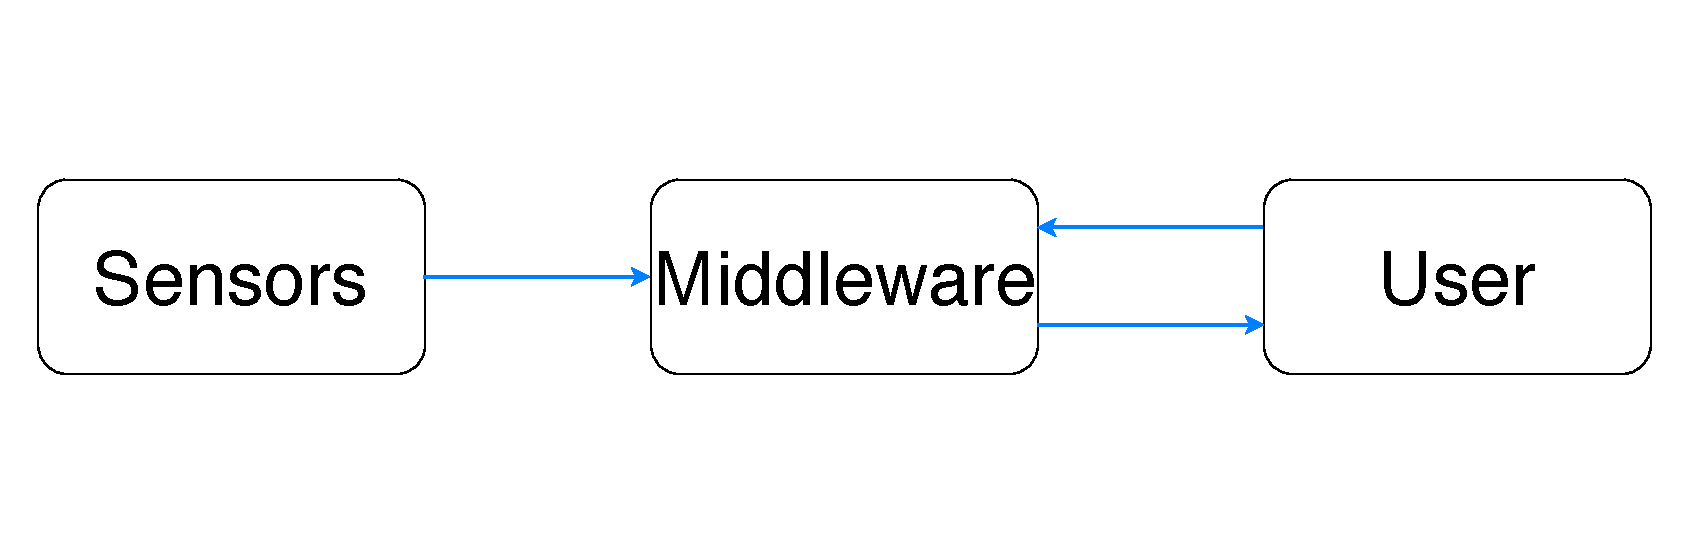
\includegraphics[width=.35\textwidth]{imgs/arq}
% \caption{Time of \texttt{get} request from server.}
% \end{figure}

Para ambos os middlewares foi implementado a mesma aplicação, onde temos as implementações disponíveis no GitHub~\cite{jcl-app}.Para avaliação do experimento, vamos considerar código propriamente dito e tempo para execução de tarefas. O cenário implementado é uma rede com um nó base (SINK) estático, dois nós sensores, há um comunicação multi-rops, onde cada sensores fazer coleta de temperatura a cada minutos e ao alcançar oito leituras, aplicamos um algoritmo de redução de dados, enviando para o sink, um pacote com dez leituras, as oito primeiras são as leituras integralmente e duas ultimas são o resultado da redução.

Podemos ver todas redes de sensores como um único componente sensores se comunicam com middleware através de um gateway, atuando unicamente como nó sensor. Já o componente usuário, pode interagir com o middleware tanto publicando quanto requisitando informações. Nossa aplicação não possui dependência com o tipo de nó sensores, podendo facilmente ser adaptada para um outra infraestrutura.

\section{Conclusions}
\subsection{Avaliação de resposta}
\begin{figure}
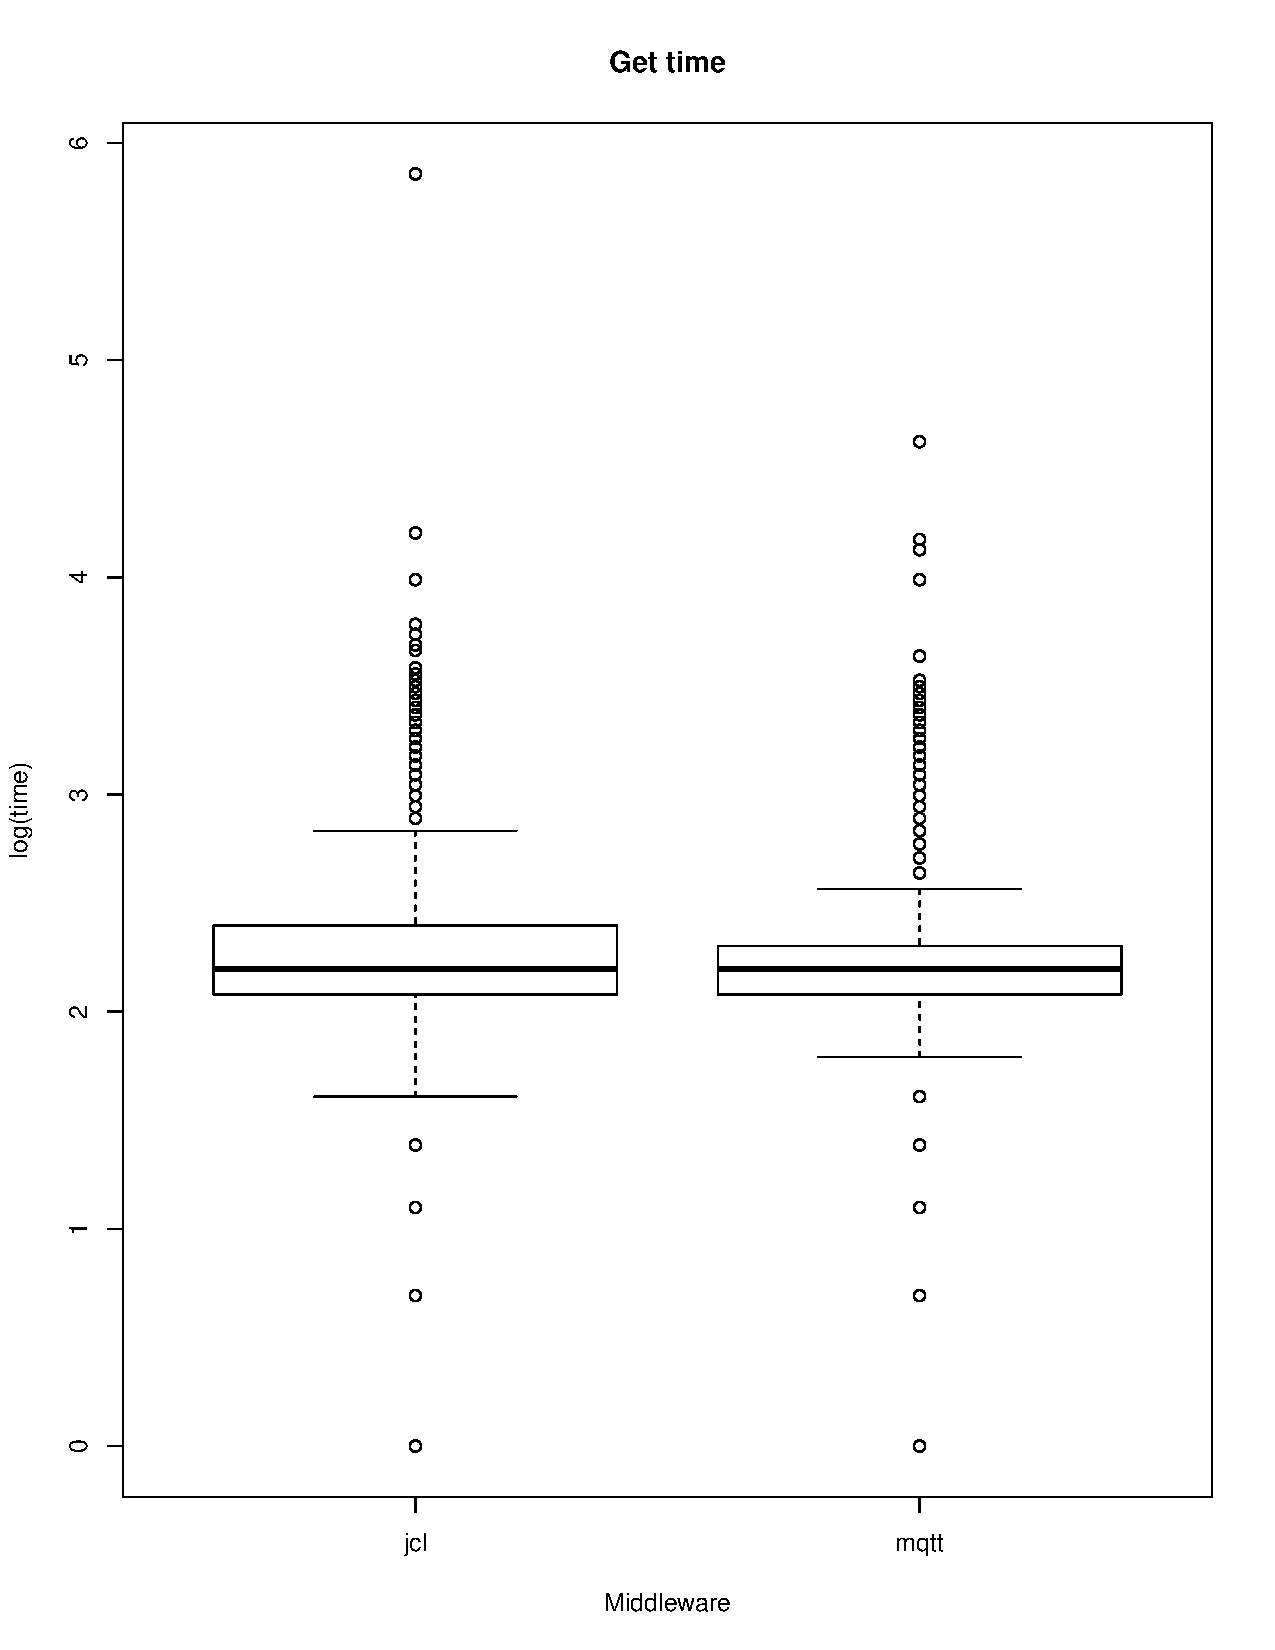
\includegraphics[width=.6\textwidth]{imgs/get-time}
\caption{Time of \texttt{get} request from server.}
\label{fig:get}
\end{figure}
\begin{figure}
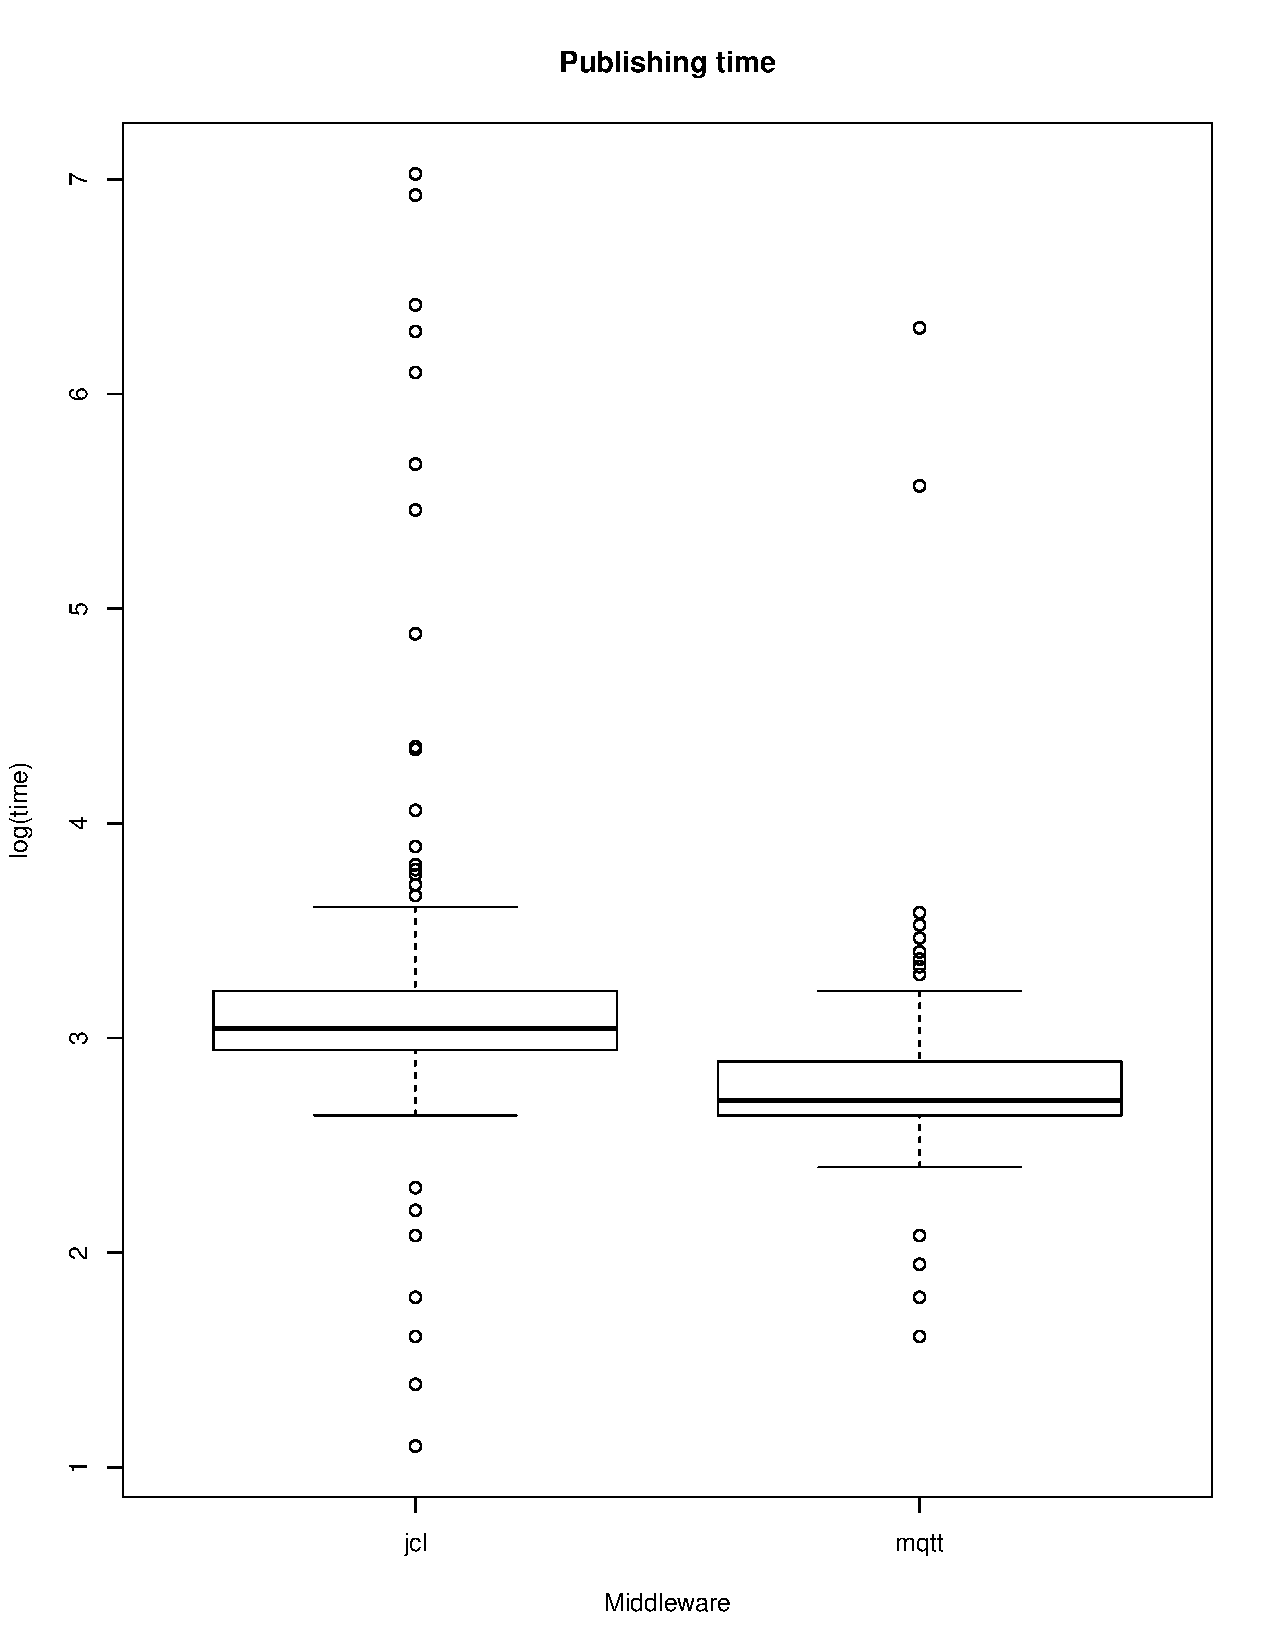
\includegraphics[width=.75\textwidth]{imgs/pub-time}
\caption{Time of \texttt{publish} sample in server.}
\label{fig:post}
\end{figure}
Durante a experimentação adotamos como métrica avaliativa de desempenho, os tempos de resposta do servidor para requisições de \textit{get} e \textit{post}. Tpmando um experimento onde conecção entre \textbf{server} e \textit{host} é feita via cabo, obtivemos os resultados mostrados nas figura~\ref{fig:get} e \ref{fig:post}

Vemos na tabela~\ref{statics}, que comparando as distribuições do JCL e MQTT para o get, percebemos que o MQTT possui menor desvio padrão em comparação com JCL, indicando assim uma maior estabilidade estatística (a distribuição possui menor espalhamento dos dados). Realizando porém o teste de hipótese, não podemos descartar a hipótese nula. 
%
Para o método post percebemos uma variação significativa em comparação do MQTT e JCL. Percebemos que, por conta da diferença do desvio padrão, o método MQTT possui uma confiabilidade estatística maior, devido ao menor espalhamento dos dados. Esses resultados podem ser evidenciados pela figura do \textit{boxplot} 

% Please add the following required packages to your document preamble:
% \usepackage{booktabs}
\begin{table}[]
\begin{tabular}{@{}ccc@{}}
\label{statics}
\toprule
          & media & desvio padrão \\ \midrule
JCL get   & 9     & 8.071343      \\
MQTT get  & 9     & 4.677674      \\
JCL post  & 21    & 76.38822      \\
MQTT post & 15    & 34.4757       \\ \bottomrule
\end{tabular}
\end{table}


\subsection{Avaliação de Código}

\begin{table}[]
\begin{tabular}{@{}ccc@{}}
\toprule
Funcionalidade            & MQTT & JCL \\ \midrule
Linhas de código          & 113  & 130 \\
Persistência de dados     & Não  & Sim \\
Suporte a Objeto Java     & Não  & Sim \\
Integração com Android    & Sim  & Sim \\
Integração com Arduino    & Sim  & Sim \\
Suporte a variável global & Não  & Sim \\
\midrule
Linhas por funcionalidade      & 56,5     & 26 \\
\bottomrule
\end{tabular}
\end{table}
\begin{table}[]
\begin{tabular}{@{}ccc@{}}
\toprule
Funcionalidade                 & MQTT     & JCL      \\ \midrule
Complexidade do código         & Fácil    & Moderado \\
Persistência de dados          & Moderado & Fácil    \\
Instalação                     & Moderado & Fácil    \\
Integrar com Android           & Fácil    & Fácil    \\
Integrar novas funcionalidades & Difícil  & Moderado \\
Documentação                   & Fácil    & Moderado \\
\bottomrule
\end{tabular}
\end{table}

\section{References}


\bibliographystyle{sbc}
\bibliography{sbc-template}

\end{document}
